\documentclass[tikz,border=10pt]{standalone}
\usetikzlibrary{shapes.geometric, arrows.meta}

\tikzstyle{startstop} = [rectangle, rounded corners, minimum width=3cm, minimum height=1cm,text centered, draw=black, fill=red!30]
\tikzstyle{process} = [rectangle, minimum width=3cm, minimum height=1cm, text centered, draw=black, fill=orange!30]
\tikzstyle{decision} = [diamond, minimum width=3cm, minimum height=1cm, text centered, draw=black, fill=green!30]
\tikzstyle{arrow} = [thick,->,>=stealth]

\begin{document}
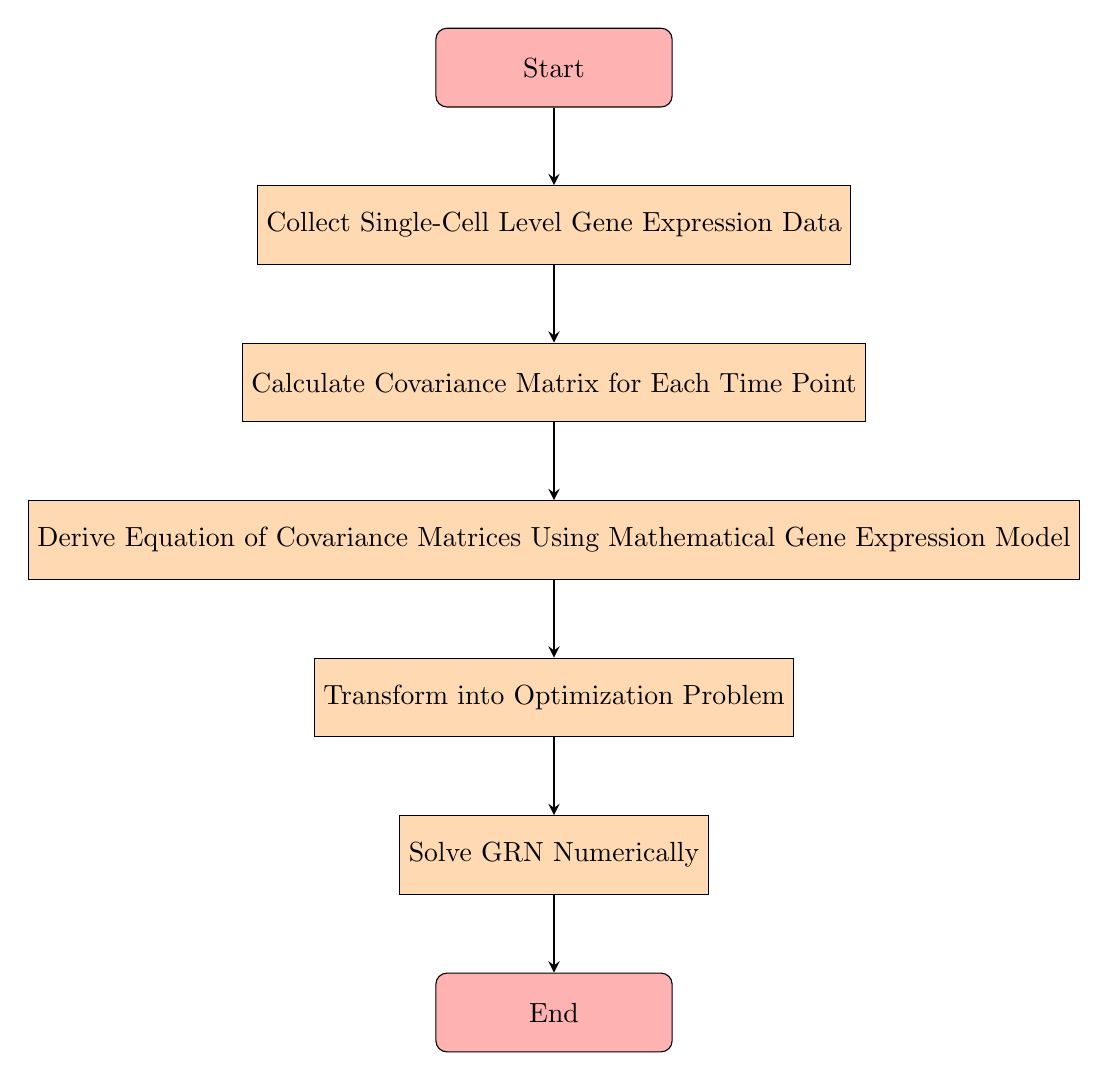
\begin{tikzpicture}[node distance=2cm]

\node (start) [startstop] {Start};
\node (data_collection) [process, below of=start] {Collect Single-Cell Level Gene Expression Data};
\node (covariance_matrix) [process, below of=data_collection] {Calculate Covariance Matrix for Each Time Point};
\node (math_model) [process, below of=covariance_matrix] {Derive Equation of Covariance Matrices Using Mathematical Gene Expression Model};
\node (optimization_problem) [process, below of=math_model] {Transform into Optimization Problem};
\node (solve_grn) [process, below of=optimization_problem] {Solve GRN Numerically};
\node (end) [startstop, below of=solve_grn] {End};

% Drawing edges
\draw [arrow] (start) -- (data_collection);
\draw [arrow] (data_collection) -- (covariance_matrix);
\draw [arrow] (covariance_matrix) -- (math_model);
\draw [arrow] (math_model) -- (optimization_problem);
\draw [arrow] (optimization_problem) -- (solve_grn);
\draw [arrow] (solve_grn) -- (end);

\end{tikzpicture}
\end{document}